\documentclass[UTF8]{ctexart}
\usepackage{listings}
\usepackage{xcolor} 
\usepackage{graphicx}
\usepackage{booktabs} %绘制表格
\usepackage{caption2} %标题居中
\usepackage{geometry}
\usepackage{array}
\usepackage{float}
\usepackage{amsmath}
\usepackage{subfigure} 
\usepackage{longtable}
\usepackage{abstract}
\pagestyle{plain} %页眉消失
\usepackage{color}
\usepackage{cases}
\usepackage{lmodern}
\usepackage[linesnumbered,ruled,vlined]{algorithm2e}  

\geometry{a4paper,left=2.5cm,right=2.5cm,top=2.5cm,bottom=2.5cm}
\lstset{
		numbers=left, %设置行号位置
		numberstyle=\tiny, %设置行号大小
		keywordstyle=\color{blue}, %设置关键字颜色
		commentstyle=\color[cmyk]{1,0,1,0}, %设置注释颜色
		escapeinside=``, %逃逸字符(1左面的键),用于显示中文
		breaklines, %自动折行
		extendedchars=false, %解决代码跨页时,章节标题,页眉等汉字不显示的问题
		xleftmargin=1em,xrightmargin=1em, aboveskip=1em, %设置边距
		tabsize=4, %设置tab空格数
		showspaces=false %不显示空格
	}
 
\title{作业: 硬币找零问题}
\author{钟琦 \\ 混合2103\quad3210103612}

\begin{document}
\maketitle
\section{问题描述}
有一定数目的面值为1、5、10、25美分的硬币,输入这些硬币的数目和需要的总金额,输出最少需要的硬币总数目。注意到硬币数目的限制,可能存在无解的情况,此时可以规定输出-1。
\section{算法思路}
本题采用动态规划的方法,对于所需要的总金额n美分,设最少需要的硬币数目为dp[n]。则根据动态规划的思路,n美分是由“(n-1)美分$+$1美分”或“(n-5)美分$+$5美分”或“(n-10)美分$+$10美分”或“(n-25)美分$+$25美分”组成的,所需硬币数dp[n]等于前者((n-1)或(n-5)或(n-10)或(n-25)美分)所需硬币数再加1。所以为使dp[n]最小,组成(n-1)、(n-5)、(n-10)、(n-25)美分需要的硬币总数目也要最少,且在这四种可能性中选择最少的硬币总数目。\par
因此,dp[n]=min(dp[n-1],dp[n-5],dp[n-10],dp[n-25])+1,初始条件为dp[0]=0,i<0时dp[i]不存在,可忽略。\par
进一步考虑硬币数目有限这一细节,产生的影响主要有两方面。一是由于硬币数量不够无法纳入动态规划:比如现有k个1美分硬币,考虑n美分由(n-1)美分+1美分组成,前面(n-1)美分中已用了k个1美分硬币,则受到1美分硬币数目限制无法再使用(n-1)美分+1美分的策略,需要将dp(n-1)从dp[n]=min(dp[n-1],dp[n-5],dp[n-10],dp[n-25])+1中剔除,即dp[n]=min(dp[n-5],dp[n-10],dp[n-25])+1;二是由于特定种类的硬币数目不够导致问题无解:比如有1、5、10、25美分硬币分别有0,0,2,0个,那对于n=15美分,2个10美分的硬币无论如何组合都无法组成15美分,会导致问题无解,此时规定返回-1。\par
展示部分求解最少硬币数的函数伪代码:\par
\begin{algorithm}[H]
    \SetAlgoLined  
    \KwData{总金额Amount,各类硬币数量coins,dp[i]}  
    \tcp{dp[i].num表示所需最少硬币数}
    \tcp{dp[i].number[t]表示最少硬币策略中所需第t类硬币数量}
    \tcp{0、1、2、3类分别对应1美分、5美分、10美分、25美分}
    \KwResult{最少所需硬币数MinCoinNumber} 
    \For{$i \leftarrow 1$ \KwTo $Amount$}{  
    \For{$t \leftarrow 1$ \KwTo $3$}{ 
      \tcp{t=0,1,2,3四种策略}
      \tcp{T=\{1,5,10,25\}}
        \If{$i$>=第$t$类硬币面值$T[t]$且$dp[i-T[t]]$有解}{
        \tcp{保证Amount=i-T[t]的问题是有解的,否则无意义}
            \If{$dp[i-T[t]].number[t]<coins[t]$}{
            \tcp{保证第t类硬币还有剩余,否则该策略行不通}
                \tcp{$n[t]$表示第t种策略下可能的dp}
                $n[t].num=dp[i-T[t]]+1$\;
                $n[t].number[t]=dp[i-T[t]]+1$\;
                \For{$j!=t$}{
                $n[t].number[j]=dp[i-T[t]]$\;
                }
            }
        }
    }
    $dp[i].num=min(n[t].num)$\;
    \tcp{选择硬币数最少的策略}
  } 
    \caption{部分MinCoinNumber函数}  
\end{algorithm}

\section{复杂度分析}
\subsection{时间复杂度}
设要求总金额为$N$情况下的最少硬币数,在利用动态规划方法计算$dp[N]$的过程中,依次计算了$dp[1]\sim dp[N]$这$N$种情况,在每种情况中,遍历了减少1美分、5美分、10美分、25美分这四种情况,且每种情况都是$O(1)$级别的平凡的判断、复制与比较,所以总时间复杂度为$O(N)$。
\subsection{空间复杂度}
向量$dp$需要开长度为$N$的空间,其余向量的长度都是有限常数大小的,且数量也是有限常数个,所以空间复杂度也为$O(N)$。
\section{测试说明}
\subsection{测试程序可行性}
输入总金额Amount,1、5、10、25美分硬币数目CoinLimit,输出solution。
\begin{itemize}
    \item [1.]输入:Amount=0,\quad CoinLimit=\{1,1,1,1\}\par
    输出:solution=0\par
    分析:金额0需要0个硬币,符合
    \item [2.]输入:Amount=40,\quad CoinLimit=\{0,0,4,1\}\par
    输出:solution=4\par
    分析:金额40若有1个25美分的硬币,则剩下的4个10美分硬币无法组成15美分,所以金额40只能由4个10美分硬币组成,符合
    \item [3.]输入:Amount=40,\quad CoinLimit=\{0,1,4,1\}\par
    输出:solution=3\par
    分析:与2不同的是多了一个5美分硬币,则40=5+10+25是最少硬币数的情况,符合
    \item [4.]输入:Amount=102,\quad CoinLimit=\{1,100,100,100\}\par
    输出:solution=-1\par
    分析:102模5余2,所以至少需要2个1美分硬币,而提供的情况只有1个1美分硬币,所以没有解,返回-1,符合
    \item [5.]输入:Amount=10000,\quad CoinLimit=\{100,2,1,399\}\par
    输出:solution=407\par
    分析:为使得所需硬币数较少,应该尽可能多地使用25美分硬币,假设全用,则$25*399=9975$,还差25美分,同理,进可能多使用10美分、5美分硬币,$5*2+1*10=20$,所以还需要5个1美分硬币,solution$=399+1+2+5=407$,符合
    \item [6.]输入:Amount=10000,\quad CoinLimit=\{1249,250,250,200\}\par
    输出:solution=-1\par
    分析:$1249*1+250*5+250*10+200*25=9999<10000$,所以无解,返回-1,符合
\end{itemize}
\subsection{测试计算效率}
\begin{itemize}
    \item [1.]当各类硬币均充足时,CoinLimit={1000000000,1000000000,1000000000,1000000000},现令Amount从0$\sim 1000000$,步长为1000,输出1000个运行时长,导出为表格(见附件1.xlxs),下为生成的散点图:
                \begin{figure}[H]
                \centering %表示居中
                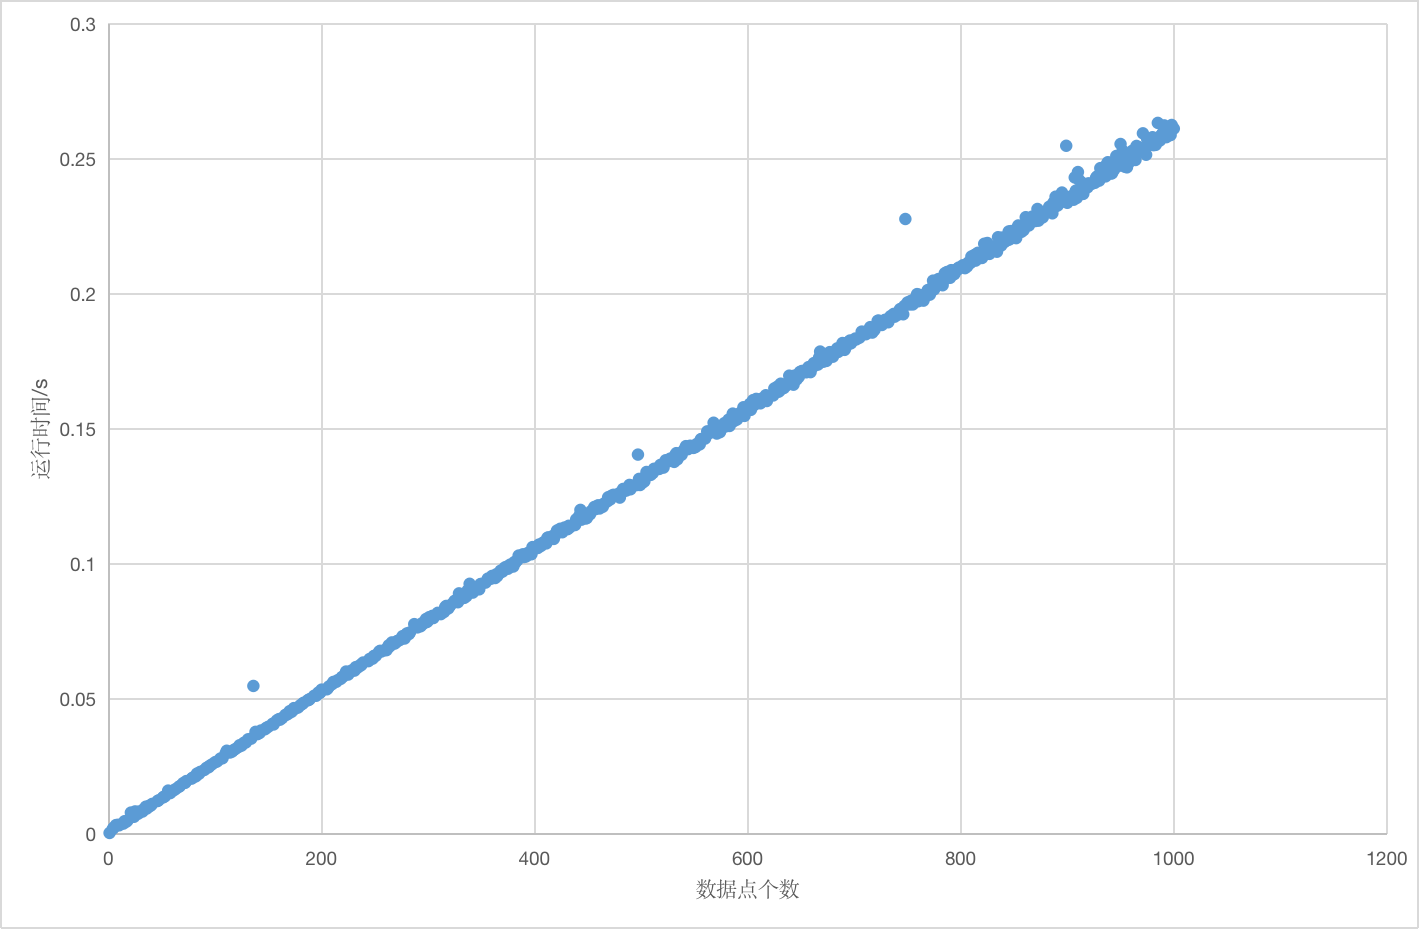
\includegraphics[width=0.8\textwidth]{Fig1.png}
                \caption{运行时间与总金额关系图}
                \label{fig1}
                \end{figure}\par
由图可知,运行时间与总金额关系曲线大致为直线,因此时间复杂度为$O(N)$,与理论结果相同。
    \item [2.]当1美分硬币不充足时,CoinLimit={1000,1000000000,1000000000,1000000000},Amount以与1相同的状态增加,下为生成的散点图:
                \begin{figure}[H]
                \centering %表示居中
                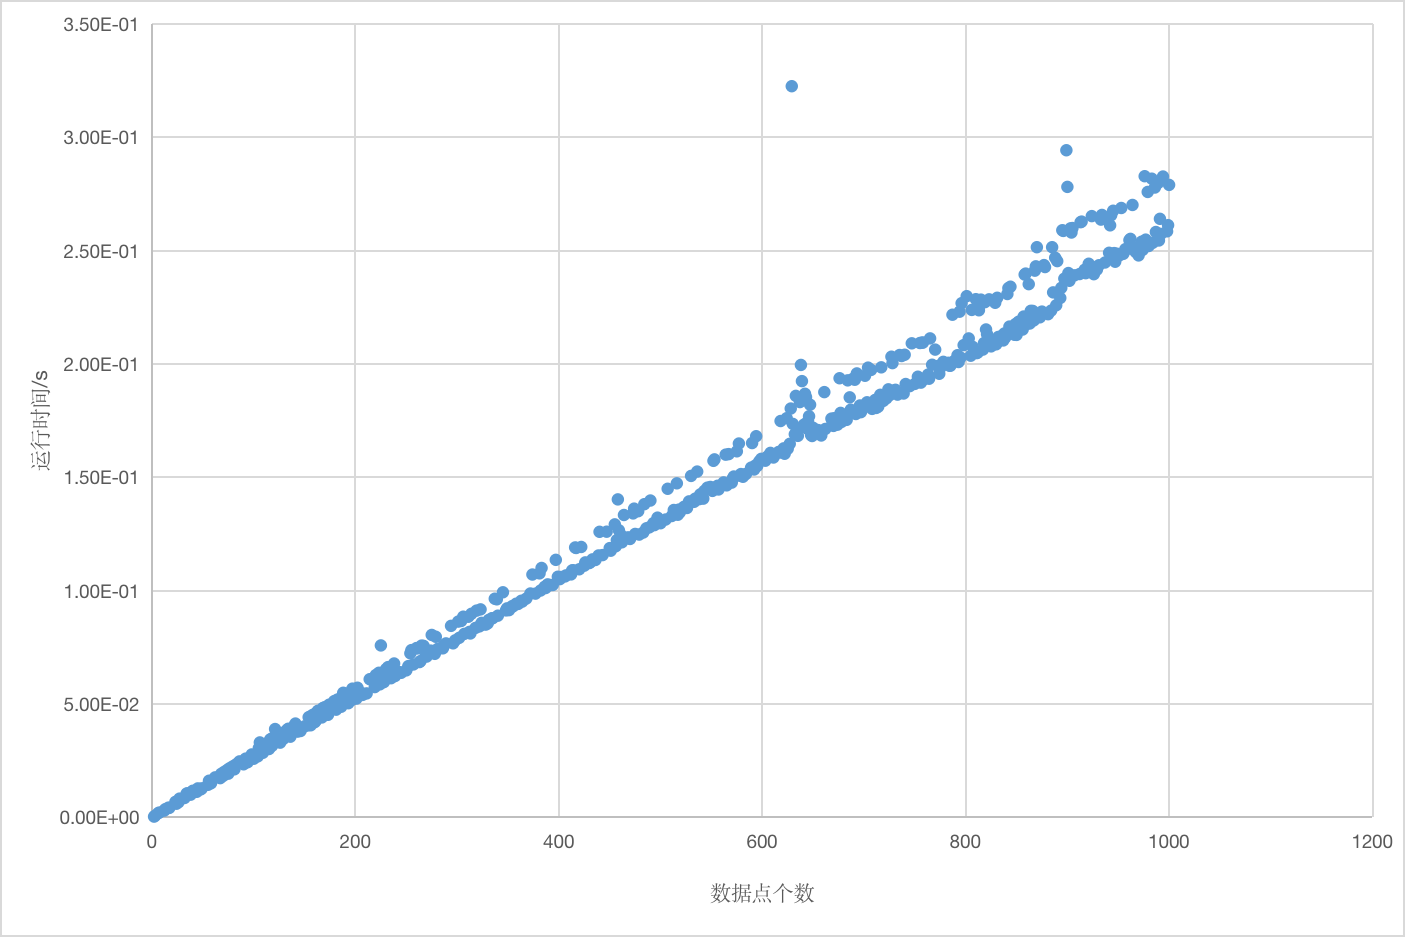
\includegraphics[width=0.8\textwidth]{Fig2.png}
                \caption{运行时间与总金额关系图}
                \label{fig2}
                \end{figure}\par
由图可知,运行时间与总金额关系曲线虽然有所分叉,都均大致为直线,因此时间复杂度为$O(N)$,与理论结果相同。
    \item [3.]当全部硬币不充足时,CoinLimit={1000,1000,1000,1000},Amount以与1相同的状态增加,下为生成的散点图:
    \begin{figure}[H]
                \centering %表示居中
                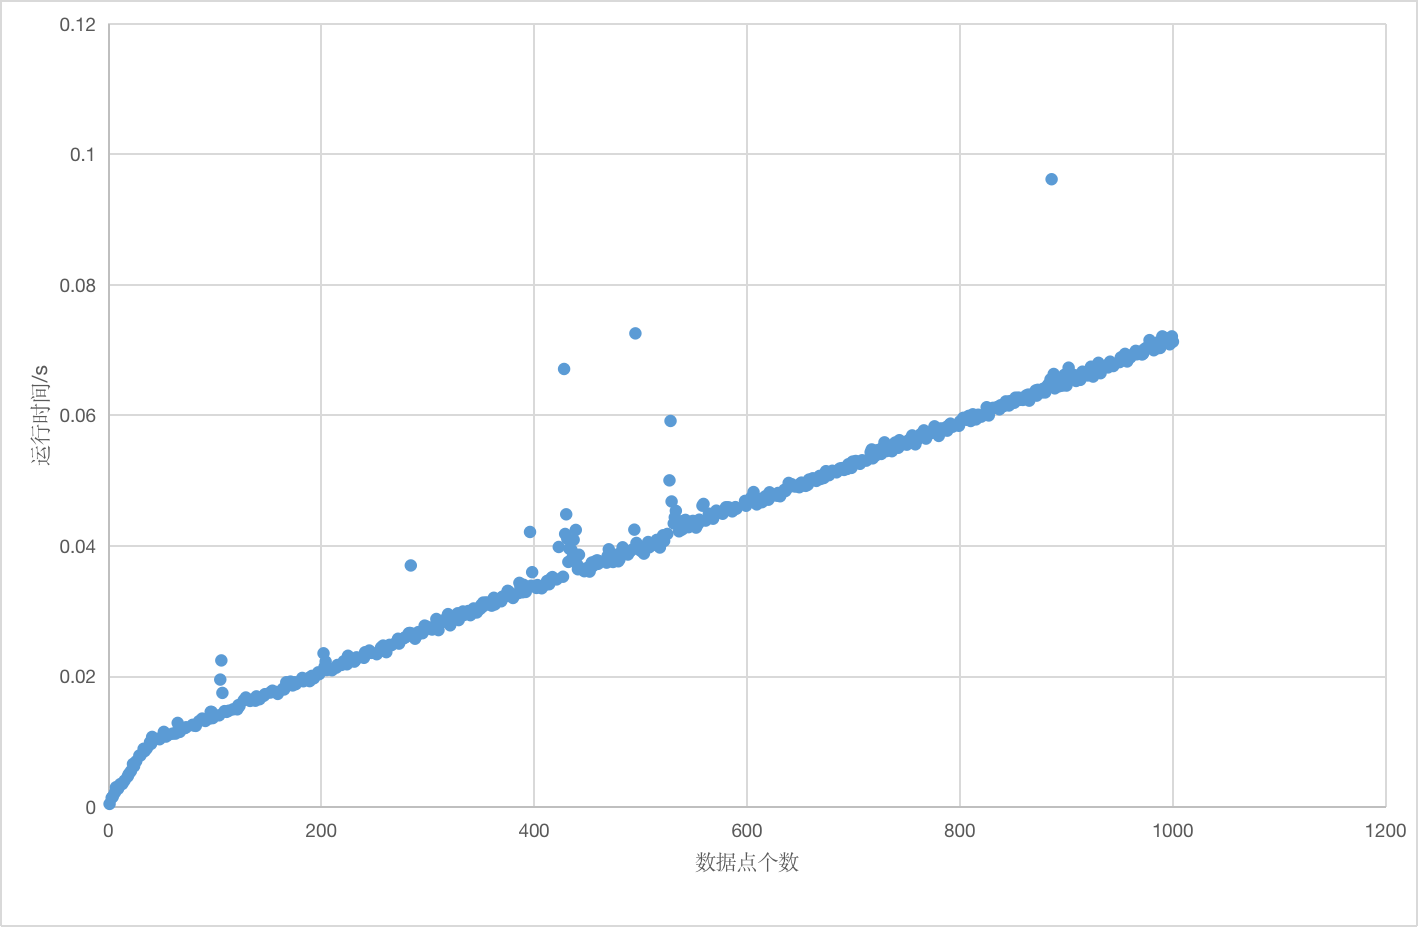
\includegraphics[width=0.8\textwidth]{Fig3.png}
                \caption{运行时间与总金额关系图}
                \label{fig3}
                \end{figure}\par
\end{itemize}
有图可知,运行时间与总金额关系曲线大致为两段斜率不同的直线组成,前一段表明硬币数目较为充足,后一段表明硬币数目不充足,但均为直线,因此时间复杂度为$O(N)$,与理论结果相同。\par
    \textbf{综上,可以得出对一般性的用例,时间复杂度为$O(N)$。}

\end{document}
